\documentclass[11pt,a4paper]{article}
\usepackage[T1]{fontenc}
\usepackage{lmodern}
\usepackage{graphicx,array,amsmath,xcolor}
\setlength{\oddsidemargin}{-2.4mm}
\setlength{\evensidemargin}{-2.4mm}
\setlength{\textwidth}{164mm}
\setlength{\topmargin}{-14mm}
\setlength{\headheight}{15pt}
\setlength{\headsep}{6mm}
\setlength{\textheight}{240mm}
\setlength{\footskip}{12mm}
\newcommand{\toprule}{\noalign{\hrule height 0.8pt}\noalign{\vskip 3pt}}
\newcommand{\midrule}{\noalign{\vskip 2pt}\noalign{\hrule height 0.4pt}\noalign{\vskip 3pt}}
\newcommand{\bottomrule}{\noalign{\vskip 3pt}\noalign{\hrule height 0.8pt}}
\usepackage{url}
\setcounter{tocdepth}{2}
\definecolor{accent}{HTML}{23877E}
\definecolor{ink}{HTML}{202C32}
\urlstyle{same}
\def\UrlBreaks{\do\/\do\-\do\_\do\?\do\=\do\.}
\makeatletter
\def\ps@reportstyle{\def\@oddhead{\small\color{ink}FIFA World Cup 2026\hfil Forecast evaluation}\let\@evenhead\@oddhead\def\@oddfoot{\small 8 October 2026\hfil\thepage}\let\@evenfoot\@oddfoot}
\long\def\@makecaption#1#2{\vskip 6pt{\small\textbf{#1.} #2\par}\vskip 4pt}
\makeatother
\setlength{\parindent}{0pt}
\setlength{\parskip}{6pt}
\setlength{\tabcolsep}{6pt}
\renewcommand{\arraystretch}{1.18}
\setlength{\textfloatsep}{12pt}
\setlength{\intextsep}{12pt}
\pagestyle{reportstyle}
\emergencystretch=2em
\begin{document}
\thispagestyle{plain}
{\color{accent}\small RESEARCH REPORT}\par
\vspace{8pt}
{\LARGE\bfseries FIFA World Cup 2026\par}
\vspace{4pt}
{\Large Simulation Forecasts Versus Actual Results\par}
\vspace{8pt}
{\small Prepared 8 October 2026\quad|\quad Four models\quad|\quad 10,000 runs per model}
\vspace{10pt}
\hrule


\begin{abstract}
This study develops and retrospectively evaluates a probabilistic simulation
framework for the FIFA World Cup 2026. The repository combines official squad
records, EAFC-style player ratings, public player statistics and national-team
strength priors to simulate complete tournaments. Three primary approaches are
compared: a Poisson baseline, a heuristic event simulator, and the same event
simulator augmented with a trained Random Forest. A legacy Random Forest run
is retained as a reference. Each saved forecast contains 10,000 tournament
realisations. Predictions are compared with FIFA's published outcomes using
stage-wise Brier scores, champion log loss and top-$k$ qualifier overlap.
Spain, the eventual champion, received title probabilities of 10.26\%, 18.18\%
and 17.11\% in the primary models, although none ranked Spain first. Heuristic
v2 achieved the lowest mean six-stage Brier score, 0.0840, compared with 0.0872
for the baseline and 0.0867 for Random Forest v2. Both v2 approaches ranked
Kylian Mbapp\'{e} first by expected goals. The analysis also identifies substantial
errors in Germany's and Brazil's projected advancement and in the prospects
of Norway and Morocco. Interpretation is limited by heterogeneous player-data
coverage, synthetic model training, and the absence of independently audited
pre-tournament publication timestamps. The results support the value of a
transparent simulation pipeline while motivating historical backtesting,
probability calibration and better source-version tracking.
\end{abstract}
\noindent\textbf{Keywords:} Monte Carlo simulation; football forecasting;
Poisson model; Random Forest; Brier score; data provenance.
\clearpage
\renewcommand{\contentsname}{Contents}
\tableofcontents
\clearpage
\listoffigures
\listoftables
\clearpage

\section{Introduction and Project Objectives}
\label{sec:introduction}
Tournament forecasting involves several sources of uncertainty: which players
are available, how team strength translates into match outcomes, and how the
draw and knockout path shape progression. A team can have the greatest chance
of winning while still being more likely to lose the tournament than to win it.
The project's central output is therefore a distribution of possible outcomes.

The repository began with an interpretable baseline and subsequently added
player-performance information, team-rating priors and a more detailed match
engine. Keeping the baseline makes it possible to ask whether additional
complexity improves the forecasts, and where it fails to do so.
\subsection{Research Questions}
\begin{enumerate}
\item How much forecast probability did each model assign to the eventual champion?
\item How accurately did the models allocate advancement probabilities across all 48 teams?
\item Did the event simulator and learned outcome layer improve on the simpler baseline?
\item Which unexpected results reveal weaknesses in team strength, tournament routing or data coverage?
\item Which conclusions are supported by saved evidence, and which require further validation?
\end{enumerate}
\subsection{Scope and Contributions}
The project covers a 48-team competition with 12 groups of four, followed by
a 32-team knockout phase. The top two teams in each group and eight best
third-place teams progress. Outputs include title and stage probabilities,
player goal and assist summaries, match-event totals, model explanations and
data-quality reports.

This report brings together the data pipeline, model definitions and evaluation
of the saved forecasts. The comparison uses stored results without retraining
on the observed tournament. The current source code documents the implemented
mechanisms, but its presence alone does not establish an immutable code version
for every June run. Frozen JSON metadata are the primary evidence for each
run's inputs, seed and model mode.
\subsection{Observed Tournament Outcome}
Spain defeated Argentina 1--0 after extra time in the final. England finished
third and France fourth. Mbapp\'{e} won the Golden Boot with 10 goals
\cite{outcome-final,outcome-standings,outcome-awards}. These observations supply
evaluation targets; they are not used to update the frozen forecasts.
\clearpage

\section{Datasets, Sources and Preparation}
\label{sec:data}
The project uses several datasets with different coverage, units and time
granularities. A player appearing in the combined file does not imply that
every player has a complete, comparable recent-season record.
\subsection{Official Squads}
The working roster contains 48 teams and 1,248 players. Its metadata identify
FIFA's English squad-list PDF, Version 1, dated 3 June 2026 at 11:30 UTC, as the
source \cite{data-fifa-squads}. The script
\path{rebuild_squads_from_fifa_pdf.py} extracts squad records; the active output
is \path{guardian_world_cup_2026_player_guide.json}. Despite its inherited
filename, the current file identifies FIFA as its squad source. The Guardian
guide is separately listed in tournament-structure provenance \cite{data-guardian}.

The source URL is a live resource: when checked for this report, the online PDF
showed a later July timestamp. That page cannot, by itself, prove the exact
contents of the locally recorded June snapshot. Archive the original file and
its checksum when reproducing or extending the study.
\subsection{EAFC Player Ratings}
The local \path{eafc26_players.csv} contains 18,405 records. Its update-date
column is 19 September 2025 throughout the file. It supplies player names,
nationality, positions, overall ratings and additional attributes. The saved
baseline reports 980 matched players and 268 fallback ratings out of 1,248:
approximately 78.5\% matched coverage and 21.5\% fallback coverage.

The export includes SoFIFA-hosted image URLs and player-path fields. These are
provenance clues, not proof of the file's original distributor. The repository
does not preserve a verified download URL, dataset release identifier or licence
for this exact CSV. Accordingly, this report cites the local artifact and
records that upstream provenance gap explicitly \cite{data-eafc}.
\subsection{Public Player-Performance Data}
The v2 input is \path{player_performance_data_statbunker.json}. Its metadata
record 19,923 source rows and 1,248 output players. Source rows can repeat a
player across competitions, seasons and table types; they are not 19,923 unique
players. StatBunker supplies the main public competition-table input, including
appearances, goals, assists, cards and goalkeeper clean sheets \cite{data-statbunker}.

Transfermarkt-derived CSVs from \path{salimt/football-datasets} supplement player
identity and performance information \cite{data-transfermarkt}. English Wikipedia
biographies and manual public-web research fill some remaining gaps
\cite{data-wikipedia}. Two players have SofaScore-derived aggregate statistics
recorded in the final metadata \cite{data-sofascore}. The final source-summary
counts are shown in Table~\ref{tab:coverage}.
\clearpage
\begin{table}[ht]
\centering\small
\caption{Primary player-statistics sources in the combined input.\label{tab:coverage}}
\begin{tabular}{lrr}
\toprule
Primary source & Players & Share (\%) \\
\midrule
Manual Web Research & 31 & 2.5 \\
Sofascore & 2 & 0.2 \\
Statbunker & 723 & 57.9 \\
Transfermarkt & 283 & 22.7 \\
Wikipedia & 209 & 16.7 \\
\bottomrule
\end{tabular}
\end{table}
\subsection{Coverage and Missingness}
StatBunker's default pages do not supply complete minutes, expected goals,
expected assists, progressive passing, tackles, saves or match ratings. Wikipedia
infoboxes often contain career totals rather than recent-season splits.
Transfermarkt supplements do not make all records equivalent in detail or
freshness. The metadata's ``complete'' flag describes populated player records;
two partial-context rows remain documented.

The research coverage report illustrates the unevenness. Panama has 18 players
below the stored 0.55 confidence threshold and 24 with zero recorded minutes;
Senegal has 14 and 25 respectively. A zero in these source-derived fields can
reflect missing evidence rather than a player having played no football.
The stored confidence measure is an engineering heuristic, not a calibrated
probability that the record is correct.

An earlier squad-quality report recorded 17 squad-shape issues and a
\texttt{needs\_refresh} status. It predates later enrichment, so it should be
treated as a historical diagnostic requiring a fresh check, not proof that all
17 issues remain in the current roster.
\subsection{National-Team Rating Priors}
The primary v2 forecasts used FIFA ranking positions transformed to an
Elo-like scale \cite{data-fifa-ranking}:
\begin{equation}
R_{\mathrm{prior}}=2170-130\ln(r),
\end{equation}
where $r$ is ranking position. The preserved fallback file records a ranking
date of 19 November 2025. This is a model-defined transformation of ranking
positions, not FIFA ranking points and not a historical World Football Elo series.

A subsequent import brought in 177 World Football Elo team records with an
as-of date of 11 June 2026 \cite{data-elo}. The import report shows coverage of all
required teams. These newer inputs are present locally, but the frozen v2 runs
evaluated here still declare the older rank-derived prior. The current input
file and the input version used by a saved result must therefore be distinguished.
\clearpage
\subsection{Tournament and Venue Context}
Groups and tournament rules are stored in
\path{world_cup_2026_simulation_structure.json}, whose metadata cite FIFA draw
information and the Guardian player guide \cite{data-draw,data-guardian}.
\path{world_cup_2026_venue_context.json} provides group-region and stage-level
context. Heat, humidity and travel-load values are modelling priors; they are
not measured match-day weather observations or a complete travel itinerary.
\subsection{Identity Resolution and Enrichment}
The preparation pipeline has four steps:
\begin{enumerate}
\item Extract squad identities, broad positions and clubs from the official list.
\item Normalize names and compare candidates using nationality, name similarity,
exact aliases and club information. Review overrides are stored separately.
\item Attach ratings and detailed positions. For unmatched EAFC players, use
role-based defaults: 68 for goalkeepers/defenders and 69 for midfielders/forwards.
\item Merge public statistics with source identity, collection status and confidence,
then construct team profiles from player records.
\end{enumerate}
Name normalization supports matching across sources; presentation should retain
the player's proper spelling. The report therefore uses Kylian Mbapp\'{e}.
Some archived records retain unaccented matching keys; those frozen identifiers
are preserved to keep the evaluation reproducible.

\path{performance_data_config.json} specifies intended collection windows,
competition weights and stage multipliers. These settings describe collection
and modelling intentions. A listed field or provider is not evidence that it
was available for every player or consumed by every saved simulation.
\subsection{Attempted and Future Data Sources}
SofaScore access was explored through direct and browser-assisted collectors;
the final source summary records only two primary SofaScore rows. Sportmonks,
API-Football/API-Sports and FootyStats have provider-ready collection paths,
but the saved input summary does not identify them as primary suppliers.

The project also attempted to fetch the international-results dataset maintained
by \path{martj42/international_results} \cite{data-historical}. The June manifest
records a failed download and no normalized results file. The stored Random
Forest training metadata consequently report zero historical rows. This
dataset is a planned input for supervised backtesting, not training evidence
for the forecasts evaluated here.
\subsection{Dataset Register}
The accompanying \path{dataset_sources.csv} records each source, the corresponding
local artifact, how it was used, and its provenance limitations. Provider URLs
are distinguished from verified URLs for the exact snapshot. The register
should be updated whenever inputs change.
\clearpage

\section{Models and Simulation Architecture}
\label{sec:models}
\subsection{Monte Carlo Tournament Simulation}
Monte Carlo simulation repeatedly draws match outcomes and plays through the
competition. For event $A$, its estimated probability after $N$ tournaments is
\begin{equation}
\widehat{P}(A)=\frac{1}{N}\sum_{i=1}^{N}\mathbf{1}\{A\text{ occurs in run }i\}.
\end{equation}
Here $N=10{,}000$ for each compared artifact. This is a count of simulated
tournaments, not machine-learning training epochs. Under independent runs,
the conditional Monte Carlo standard error is approximately
$\sqrt{\widehat p(1-\widehat p)/N}$. For a 20\% title probability it is about
0.4 percentage points. Running more simulations reduces this sampling noise;
it does not repair biased ratings or inaccurate football assumptions.

\subsection{Model 1: EAFC--Poisson Baseline}
The baseline in \path{simulate_world_cup.py} builds a position-aware starting
XI, a top-18 group and a full-squad mean. Team strength is
\begin{equation}
S=0.62\overline R_{\mathrm{XI}}+0.28\overline R_{18}
  +0.10\overline R_{\mathrm{squad}}.
\end{equation}
For strength difference $\Delta=S_A-S_B$, expected goals are
\begin{align}
\lambda_A&=\operatorname{clip}(1.28+0.045\Delta,\,0.25,\,3.4),\\
\lambda_B&=\operatorname{clip}(1.28-0.045\Delta,\,0.25,\,3.4).
\end{align}
The match score is sampled using Poisson goal counts. The baseline is useful
because its rating-to-score relationship is simple to inspect. Its limitations
include static strength, role-based fallback ratings and limited representation
of changing match state. Its stored metadata describe knockout seeding based on
group-stage performance, whereas v2 uses constrained bracket routing; differences
between model results therefore reflect more than the learning algorithm alone.

\subsection{Shared v2 Event Engine}
The v2 implementation adds position-sensitive player-performance adjustments,
lineup selection and separate attack, midfield, defence, goalkeeper and
possession profiles. Match context includes team priors, host advantage,
rest, accumulated fatigue, lineup replacements and venue/travel assumptions.
Regulation time is compressed into nine simulated ticks and extra time into
three. Possession, fouls, cards, removals, substitutions, set pieces and game
state can affect scoring; tied knockout matches proceed to extra time and
penalties. The engine carries player state through the tournament and supports
CPU-parallel tournament batches.
\clearpage
\subsection{Model 2: Heuristic Event Simulator}
The heuristic mode uses 96 deterministic, seeded rule-based votes to adjust
attack share, tempo, discipline and possession. The thresholds are hand-built
mechanics, not trees learned from observed match outcomes. The aggregate
modifiers feed the expected-goal calculation before the event engine produces
the match result.

This version asks whether additional team and match context improves on the
baseline without fitting a supervised outcome classifier. It is more expressive,
but the additional coefficients and constraints also introduce assumptions
requiring validation. Both v2 modes retain this heuristic component.
\subsection{Model 3: Random Forest-Augmented Event Simulator}
The learned component is a scikit-learn Random Forest classifier with outcomes
$A$ win, draw and $B$ win. The inspected implementation uses 96 trees, maximum
depth 8, at least 6 samples per leaf, balanced-subsample class weighting and a
fixed seed. Its 21 inputs cover strength and unit differences, discipline and
data confidence, host/rest/fatigue context, venue/travel conditions and tournament
stage information. A model feature need not represent directly measured evidence:
several inputs are derived priors.

The forest modifies the event simulator rather than replacing it. Let
$s_{\mathrm{base}}$ be the engine's attacking share and $p_A,p_D,p_B$ the forest's
outcome probabilities. The pre-clipping blend is
\begin{equation}
s_A=0.72s_{\mathrm{base}}+
0.28\frac{p_A}{\max(0.01,p_A+p_B)}.
\end{equation}
The draw probability also adjusts total expected goals. Consequently, the final
tournament probabilities reflect the combined rating model, heuristic rules,
learned adjustment and stochastic event engine.
\subsection{Synthetic Training and Its Implications}
The stored forest uses 6,768 synthetic rows and no historical match rows. This
count follows from $48\times47$ ordered team pairings across three contexts.
The generator perturbs features and samples outcome labels from a hand-defined
probability function involving team strength, unit matchups and context.

The model therefore learns the behaviour of the synthetic generator. Good
performance on held-out synthetic rows does not establish real-match accuracy.
The saved RF run's 0.7301 accuracy is measured on its training data and must not
be presented as a 73.01\% World Cup prediction success rate. The code supports
historical training when enough usable labels exist; that path was not active
for these artifacts.
\clearpage
\subsection{Legacy Reference and Experimental Controls}
The legacy RF run uses squad-proxy Elo rather than the national-team rank prior.
It is retained to expose the effect of earlier assumptions, but excluded from
the primary model-average comparison. Different seeds, bracket mechanics,
priors and context versions mean the stored runs are not a controlled ablation
of one factor at a time.
\begin{table}[ht]
\centering\small
\caption{Frozen forecast inventory. Seeds are identifiers, not dates of publication.}
\begin{tabular}{lrrl}
\toprule
Model & Runs & Seed & Rating prior \\
\midrule
EAFC baseline & 10000 & 20260605 & EAFC only \\
Heuristic v2 & 10000 & 20260620 & FIFA rank-derived \\
Random Forest v2 & 10000 & 20260621 & FIFA rank-derived \\
Legacy RF & 10000 & 20260618 & Squad proxy \\
\bottomrule
\end{tabular}
\end{table}
\subsection{Additional Research Models}
The research pipeline also benchmarks L2 logistic regression, sigmoid-calibrated
logistic regression, Extra Trees, histogram gradient boosting and an ensemble
weighted by inverse validation log loss. Logistic regression provides a linear
reference; calibration adjusts probability outputs; the tree ensembles explore
nonlinear feature interactions. These are diagnostic experiments, not five
additional frozen tournament forecasts in this retrospective comparison.

The stored research split contains 5,076 training rows and 1,692 test rows from
the synthetic frame. Calibrated logistic regression has log loss 0.75862;
Random Forest has 0.79449. These numbers use synthetic targets and are not
comparable to champion log loss on the actual tournament.

The ensemble chooses its weights using the same held-out results on which the
ensemble is then scored. Its reported score is consequently not an independent
final test. Future work should separate fitting, calibration, model selection
and final chronological evaluation. Random splitting of related synthetic
team pairings is also weaker evidence than held-out tournaments or dates.
\subsection{Feature Importance and Explainability}
The earlier feature study uses tree importance, permutation importance,
feature-group ablation, partial dependence, individual conditional expectation
and local feature occlusion. Squad-rating difference, possession difference and
attack-versus-defence are leading signals in the stored permutation results.
Unit-matchup ablation yields the largest reported validation log-loss increase,
approximately 0.0228.

These results explain sensitivity within the synthetic modelling framework;
they do not establish causal determinants of real football outcomes. The
tournament-level RF ablation uses only 30 runs per scenario and leaves the
hand-built expected-goal mechanics active. Those exploratory results are not
equivalent to full-engine ablation or a 10,000-run controlled comparison.
\clearpage



\section{Evaluation Design}
The comparison joins frozen forecast percentages with binary indicators of actual
advancement for each of the 48 teams. The analysis verifies that the comparison
CSVs match the original JSON outputs and that the observed stage memberships
are nested correctly. FIFA's knockout results supply advancement membership
\cite{outcome-knockouts}. The main comparison contains 1,536 team-stage rows:
four models, 48 teams and eight reported outcomes per team.


\begin{figure}[ht]\centering
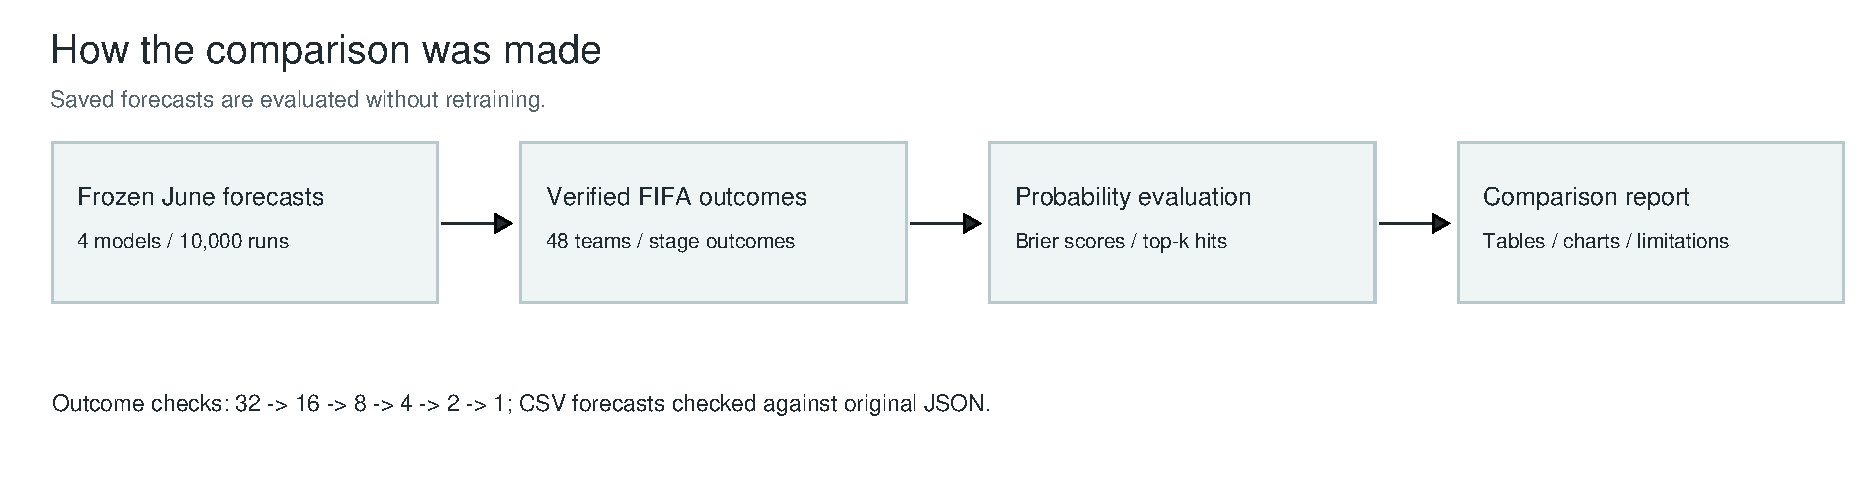
\includegraphics[width=\linewidth]{figures/evaluation_workflow.pdf}
\caption{Workflow for evaluating saved forecasts against sourced tournament outcomes.}
\end{figure}

\subsection{Probability Scores}
For team $t$ at stage $s$, let $p_{t,s}$ be the forecast probability and
$y_{t,s}\in\{0,1\}$ indicate whether that team reached the stage.
\begin{align}
\mathrm{BS}_s &= \frac{1}{48}\sum_{t=1}^{48}(p_{t,s}-y_{t,s})^2,\\
\mathrm{Skill}_s &= 1-\frac{\mathrm{BS}_s}{q_s(1-q_s)},\qquad q_s=\frac{k_s}{48},\\
\mathrm{LL}_{\mathrm{champion}} &= -\ln p_{\mathrm{Spain},\mathrm{champion}}.
\end{align}
Lower Brier score and log loss are better. Positive skill indicates improvement
over a uniform stage probability. The categorical champion Brier score is the
\emph{sum} across 48 outcomes; advancement Brier scores are \emph{means}.

The combined advancement score is the equally weighted mean over six stages:
last 32, last 16, quarter-finals, semi-finals, final and champion. Third- and
fourth-place outcomes are reported separately.
\subsection{Top-$k$ Overlap}
For a stage admitting $k$ teams, the analysis counts how many of the $k$ highest
forecast teams actually reached it. Equal probabilities use alphabetical ordering.
This ranking measure complements probability scores but does not assess calibration.
\clearpage
\section{Championship Forecasts}
Spain had substantial probability in each primary forecast, but no primary model
selected Spain as its favourite. A likely contender winning is compatible with
the forecast even when the highest-ranked team's prediction is incorrect.


\begin{figure}[ht]\centering
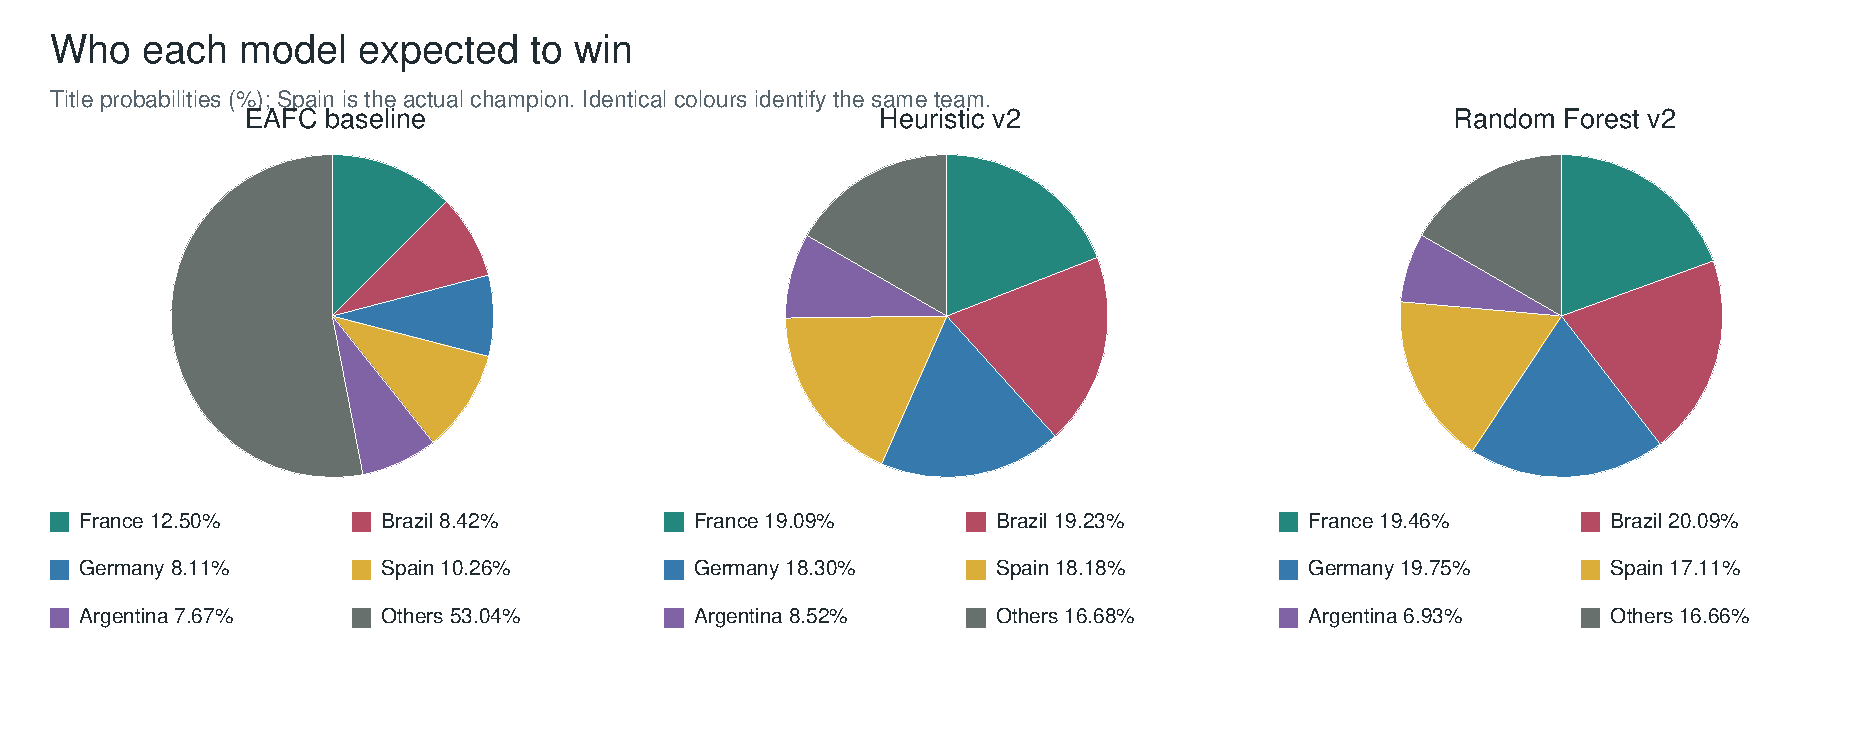
\includegraphics[width=\linewidth]{figures/champion_probability_pies.pdf}
\caption{Title-probability distributions for the three primary models. Each pie totals 100\%; Others combines all teams outside the five named contenders.}
\end{figure}

\begin{table}[ht]
\centering\small
\caption{Forecast support for the actual champion. Legacy RF is a reference model.}
\begin{tabular}{llrrrr}
\toprule
Model & Favourite & Spain rank & Spain (\%) & Log loss & Brier sum \\
\midrule
EAFC baseline & France & 2 & 10.26 & 2.277 & 0.864 \\
Heuristic v2 & Brazil & 4 & 18.18 & 1.705 & 0.790 \\
Random Forest v2 & Brazil & 4 & 17.11 & 1.766 & 0.817 \\
Legacy RF & France & 2 & 14.38 & 1.939 & 0.870 \\
\bottomrule
\end{tabular}
\end{table}

\begin{figure}[ht]\centering
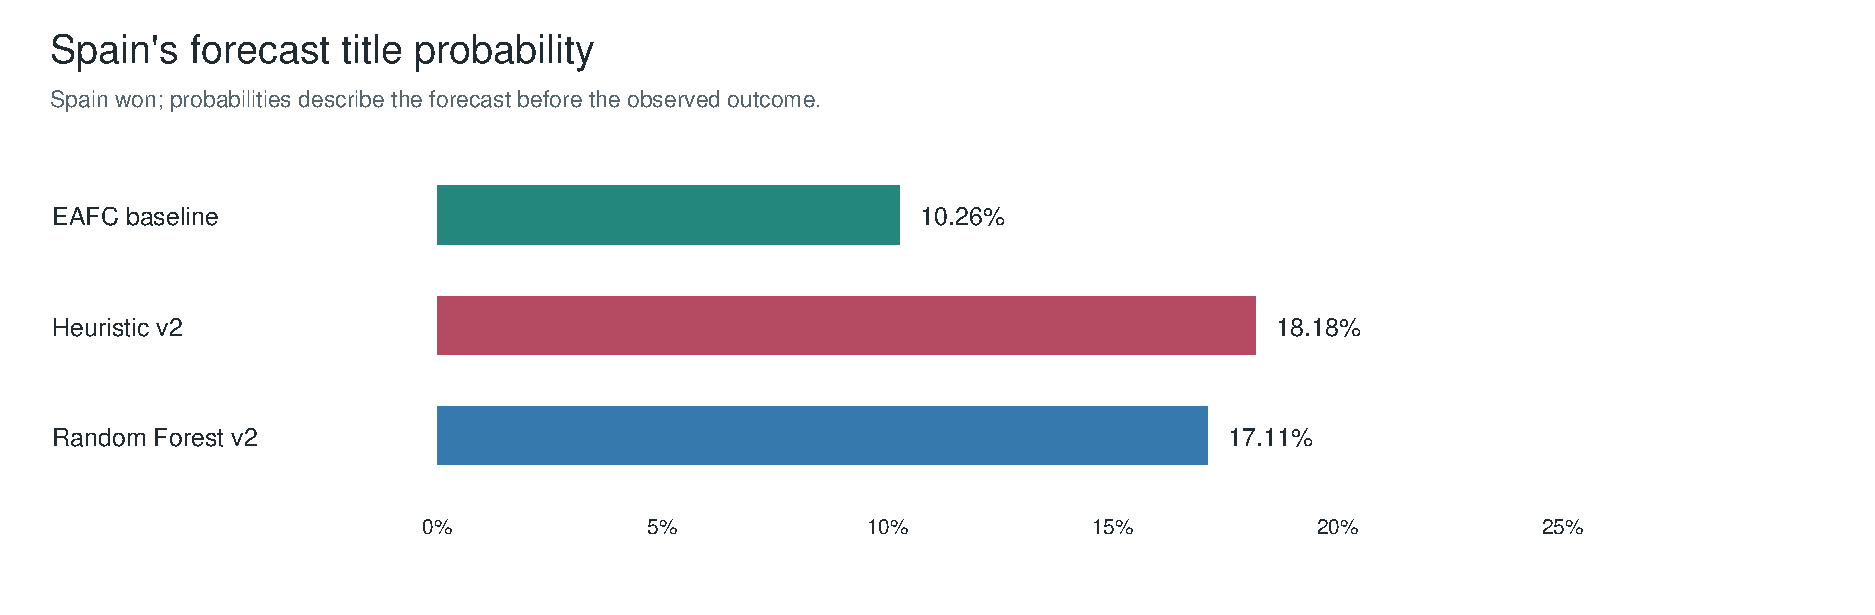
\includegraphics[width=0.9\linewidth]{figures/spain_title_probability.pdf}
\caption{Spain's title probability across the primary models.}
\end{figure}

\clearpage
\section{Advancement Accuracy}
The richer heuristic model improves the combined score relative to the baseline,
but the improvement is not uniform across stages. The baseline has lower Brier
error at the quarter-final, semi-final and final stages.


\begin{figure}[ht]\centering
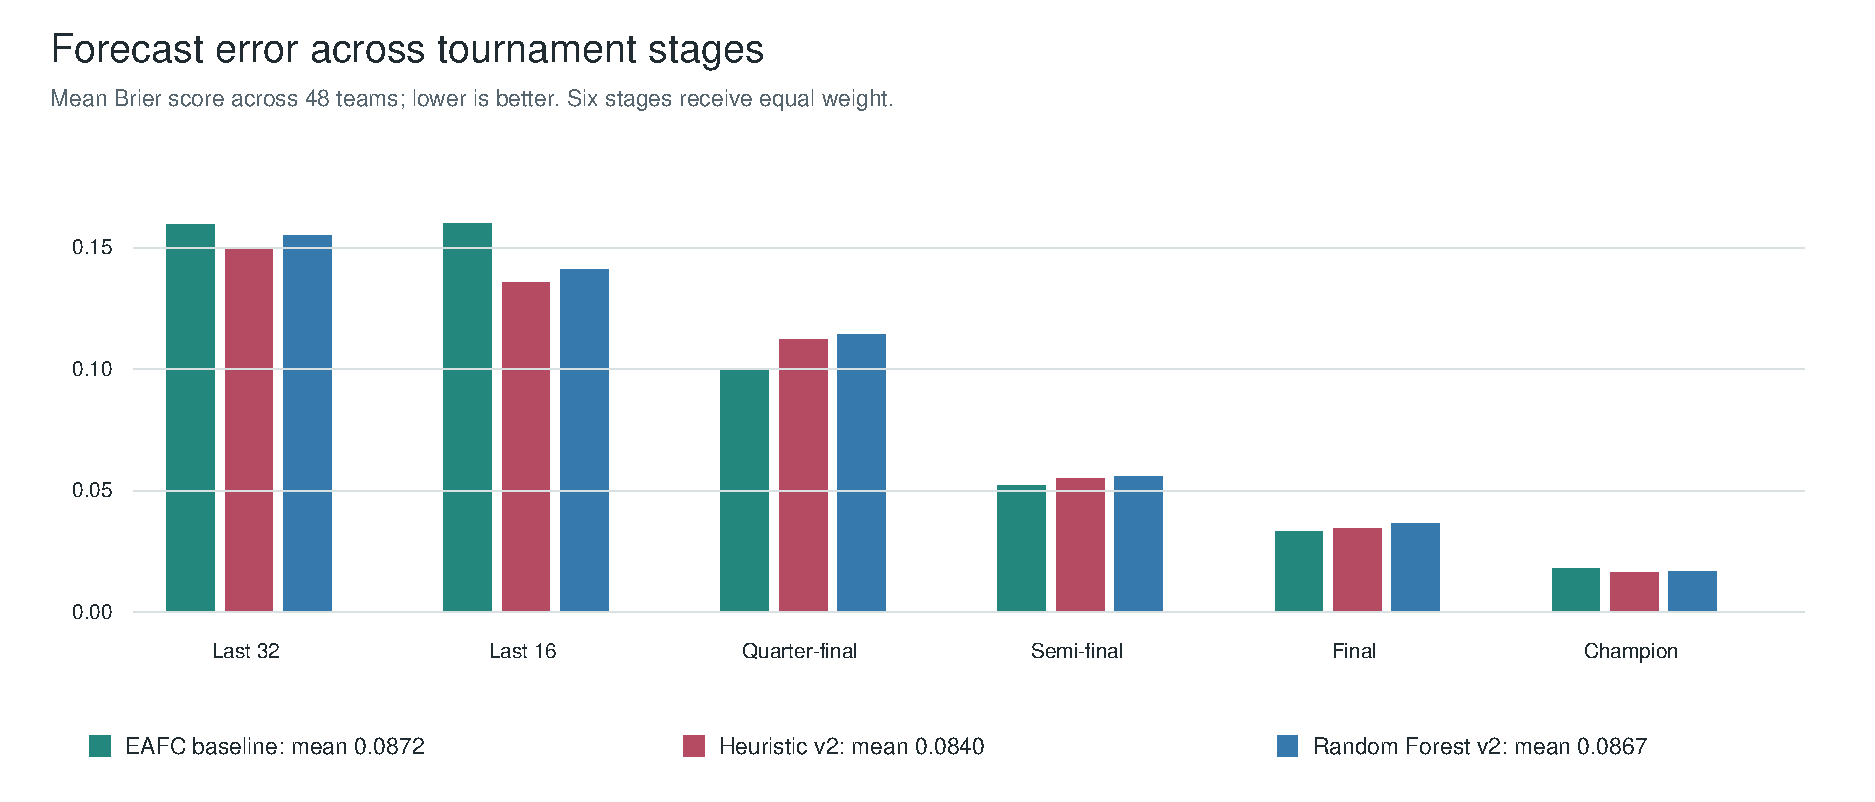
\includegraphics[width=\linewidth]{figures/stage_accuracy.pdf}
\caption{Stage-wise mean Brier scores. Compare models within a stage because the stage base rates differ.}
\end{figure}

\begin{table}[ht]
\centering\small
\caption{Advancement error and top-ranked qualifier overlap across the three primary models.}
\begin{tabular}{lrrrl}
\toprule
Stage & Baseline & Heuristic & RF & Top-$k$ hits (B / H / RF) \\
\midrule
Last 32 & 0.1594 & 0.1497 & 0.1551 & 27/32 / 27/32 / 27/32 \\
Last 16 & 0.1599 & 0.1357 & 0.1411 & 11/16 / 11/16 / 11/16 \\
Quarter-final & 0.1004 & 0.1124 & 0.1143 & 4/8 / 4/8 / 4/8 \\
Semi-final & 0.0521 & 0.0552 & 0.0559 & 2/4 / 2/4 / 2/4 \\
Final & 0.0332 & 0.0345 & 0.0366 & 1/2 / 0/2 / 0/2 \\
Champion & 0.0180 & 0.0165 & 0.0170 & 0/1 / 0/1 / 0/1 \\
Third place & 0.0190 & 0.0187 & 0.0174 & 0/1 / 0/1 / 0/1 \\
Fourth place & 0.0197 & 0.0211 & 0.0211 & 0/1 / 0/1 / 0/1 \\
\bottomrule
\end{tabular}
\end{table}

\begin{table}[ht]
\centering\small
\caption{Equal-weight combined advancement scores; lower is better.}
\begin{tabular}{lr}
\toprule
Primary model & Mean six-stage Brier \\
\midrule
EAFC baseline & 0.0872 \\
Heuristic v2 & 0.0840 \\
Random Forest v2 & 0.0867 \\
\bottomrule
\end{tabular}
\end{table}

\clearpage
\section{Where Forecasts and Outcomes Diverged}


\begin{figure}[ht]\centering
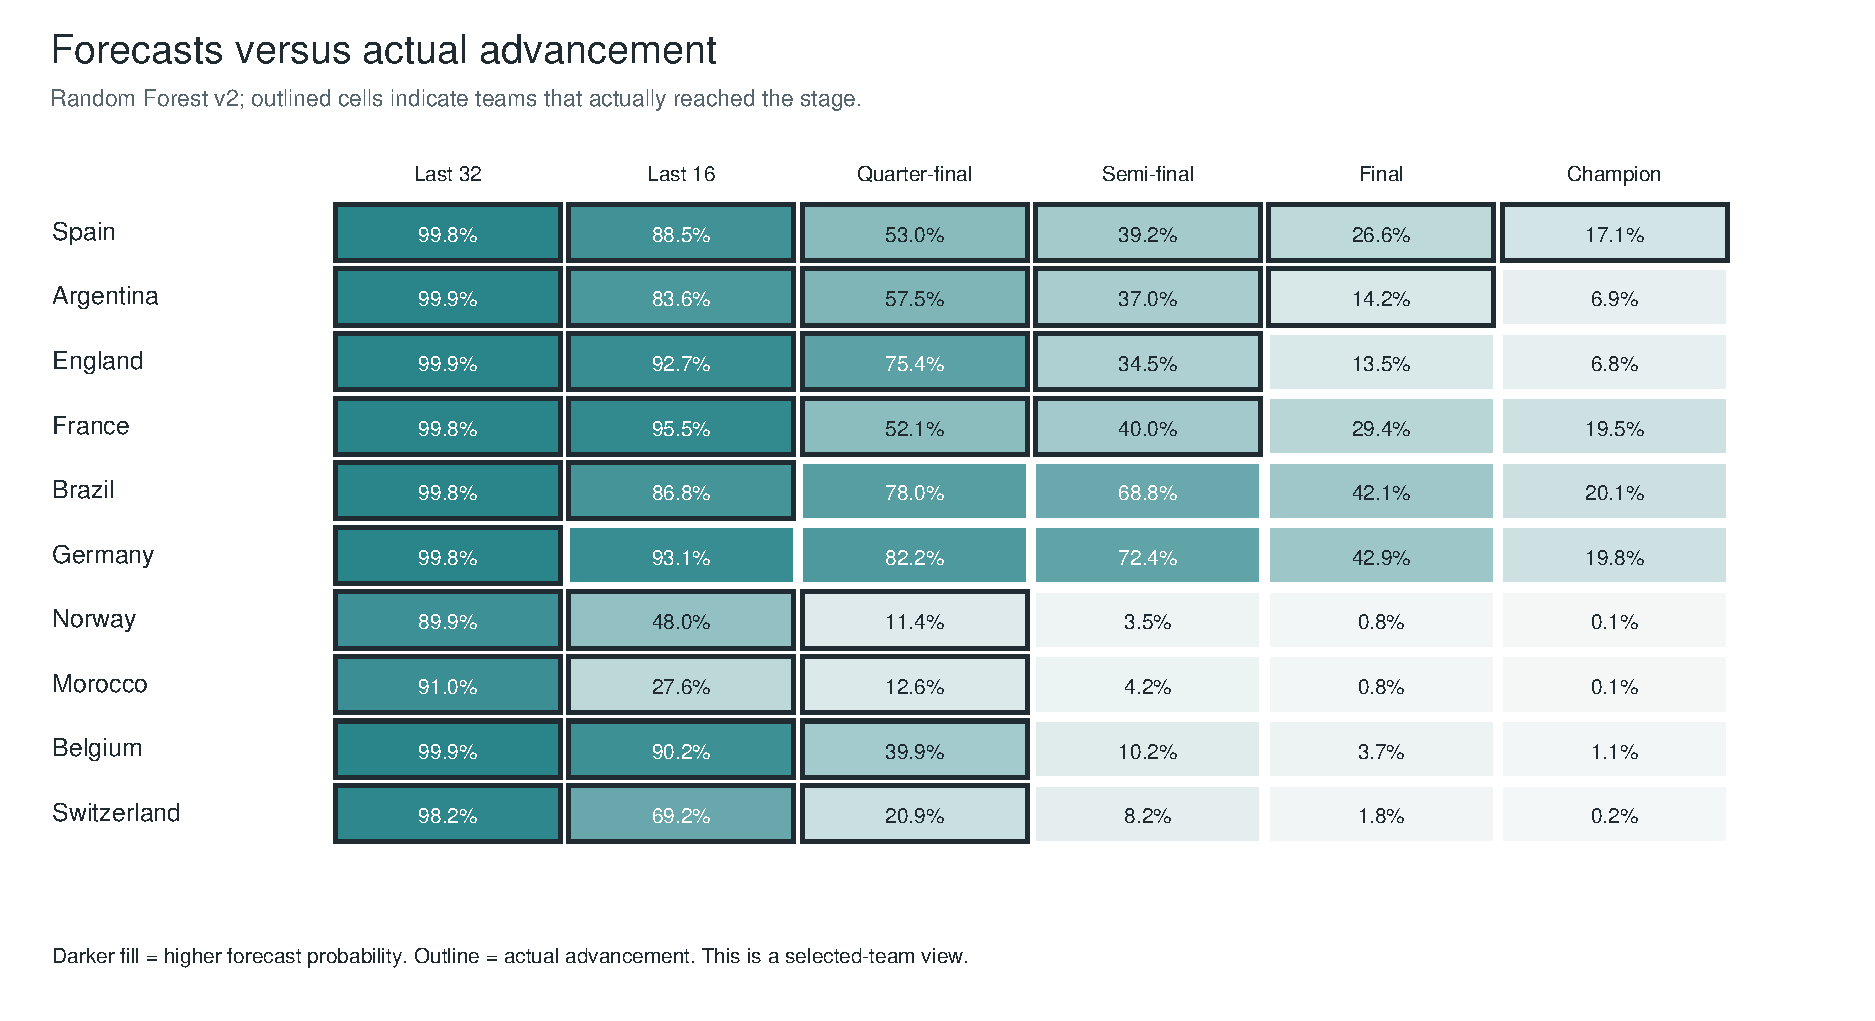
\includegraphics[width=\linewidth]{figures/forecast_outcome_heatmap.pdf}
\caption{Random Forest v2 probabilities for selected teams. Outlined cells indicate actual advancement; darker fills indicate higher forecast probability.}
\end{figure}

Germany exited in the last 32 and Brazil in the last 16 despite high v2
advancement probabilities. Norway, Morocco, Belgium and Switzerland reached
the quarter-finals. The selected-team heatmap illustrates both overestimation
of highly rated contenders and underestimation of unexpected progress.

These discrepancies suggest reviewing upset frequency, bracket effects and
player-data coverage. The observed outcomes alone cannot identify which
mechanism caused a forecast error.


\begin{table}[ht]
\centering\small
\caption{Eight largest absolute discrepancies among primary-model quarter-final, semi-final and final forecasts.}
\begin{tabular}{lllrl}
\toprule
Model & Team & Stage & Forecast (\%) & Reached? \\
\midrule
Heuristic v2 & Norway & Quarter-final & 10.38 & Yes \\
Random Forest v2 & Norway & Quarter-final & 11.41 & Yes \\
Random Forest v2 & Morocco & Quarter-final & 12.61 & Yes \\
EAFC baseline & Argentina & Final & 13.86 & Yes \\
Random Forest v2 & Argentina & Final & 14.16 & Yes \\
Heuristic v2 & Morocco & Quarter-final & 15.66 & Yes \\
Heuristic v2 & Argentina & Final & 17.25 & Yes \\
EAFC baseline & Spain & Final & 17.77 & Yes \\
\bottomrule
\end{tabular}
\end{table}

\clearpage
\section{Player Scoring and Interpretation}
Kylian Mbapp\'{e} won the Golden Boot with 10 goals. Both primary v2 models ranked
him first by expected aggregate goals; the baseline ranked him second.


\begin{table}[ht]
\centering\small
\caption{Expected scoring rank and mean goals versus one observed tournament.}
\begin{tabular}{lrrr}
\toprule
Model & Mbapp\'{e} rank & Mean goals & Actual goals \\
\midrule
EAFC baseline & 2 & 1.446 & 10 \\
Heuristic v2 & 1 & 2.946 & 10 \\
Random Forest v2 & 1 & 2.904 & 10 \\
Legacy RF & 1 & 3.467 & 10 \\
\bottomrule
\end{tabular}
\end{table}

Expected goals over many simulated tournaments and observed goals in a single
tournament are different quantities. A mean of approximately three goals does
not predict that the player must score three. Similarly, a ranking by expected
goals is not the probability of winning the Golden Boot. This comparison is
descriptive; award forecasting would require a separate probability calculation.
\section{Provenance, Limitations and Next Steps}
\subsection{Forecast Provenance}
Each model ran 10,000 tournaments. The two primary v2 artifacts used
FIFA-rank-derived Elo-scale priors, rather than the raw World Football Elo data
imported later. Random Forest training used synthetic profile calibration;
historical-match predictive accuracy was not established.

Seeds that resemble dates are random-number seeds, not creation timestamps.
The artifacts were saved around the start of the tournament and the v2 files
were last modified on 11 June. Local timestamps do not prove publication before
kickoff. This report therefore evaluates saved forecasts retrospectively.
\subsection{Statistical and Data Limits}
Advancement indicators are dependent; six stages across 48 teams are not 288
independent observations. One tournament cannot establish calibration or model
superiority. Wilson intervals in prior reports measure Monte Carlo sampling
error conditional on model assumptions, not uncertainty about those assumptions.

Saved outputs do not supply probabilities for every actual match or every
player. Match-level log loss and full player-goal errors are outside scope.
Group-stage exits are inferred from absence in the verified last-32 field.
Rankings among teams eliminated at the same stage are not inferred.
\clearpage
\subsection{Recommended Research Work}
\begin{enumerate}
\item Backtest several historical tournaments using information available at each match date.
\item Calibrate goal, draw and upset rates on real international results.
\item Review bracket routing and concentration of probability on stronger teams.
\item Improve low-confidence player coverage and model Golden Boot probabilities separately.
\item Publish dated forecast snapshots before future tournaments.
\end{enumerate}
\subsection{Reproducibility}
Run \texttt{python compare\_simulation\_with\_actuals.py} from the repository root.
The analysis regenerates CSV score tables, Markdown and HTML reports, charts
and this LaTeX source. Compile the source from the report folder using
\texttt{pdflatex -jobname=comprehensive\_report}\par
\texttt{comparison\_report.tex}\par
Repeat until contents pages and cross-references settle.

Supporting data: \texttt{actual\_outcomes.json}, \texttt{model\_scores.csv},\par
\texttt{team\_stage\_comparison.csv}, \texttt{champion\_comparison.csv},\par
\texttt{scorer\_comparison.csv}, \texttt{prediction\_sha256.json}.\par
The hashes identify the frozen inputs. Figure PDFs are supplied in the
\texttt{figures/} folder.
\section{Conclusion}
The project establishes an inspectable chain from data collection to simulated
tournaments and retrospective evaluation. Spain was a credible contender in
every primary forecast, but the favoured team was wrong in each case. Heuristic
v2 achieved the best combined advancement score on this tournament, while the
baseline performed better at some later stages. The RF extension did not deliver
a consistent improvement over the heuristic engine.

The most useful next step is stronger validation: chronologically separated
historical data, measured match context, controlled model comparisons and
published forecast snapshots. These improvements would make it possible to
distinguish the benefits of richer football information from the effects of
hand-set assumptions and synthetic training.


\clearpage
\addcontentsline{toc}{section}{References and Data Sources}
\renewcommand{\refname}{References and Data Sources}
\begin{thebibliography}{99}
\small\raggedright
\setlength{\itemsep}{3pt}
\setlength{\parskip}{1pt}
\setlength{\parsep}{0pt}
\bibitem{data-fifa-squads} FIFA. \emph{FIFA World Cup 2026 squad lists, English}.
Local metadata identify Version 1, 3 June 2026; live URL may change.
\par\url{https://fdp.fifa.org/assetspublic/ce281/pdf/SquadLists-English.pdf}
\bibitem{data-eafc} Local EAFC 26 ratings export. \path{eafc26_players.csv}.
18,405 records; update-date field 19 September 2025. Original download URL,
distributor and licence not preserved. SoFIFA-hosted image links are recorded
in the file but do not establish its full provenance.
\bibitem{data-statbunker} StatBunker. Public football player competition tables.
Provider and a concrete endpoint recorded in the collection manifest:
\par\url{https://www.statbunker.com/}
\par\url{https://www.statbunker.com/competitions/PlayerStandings?comp_id=776}
\bibitem{data-transfermarkt} salimt. \emph{football-datasets}. Transfermarkt-derived
CSV supplement; the local enrichment manifest identifies profile, performance,
national-team and related CSV files.
\par\url{https://github.com/salimt/football-datasets}
\bibitem{data-wikipedia} English Wikipedia / MediaWiki. Player-biography infoboxes.
Individual article URLs are stored in player records; the collector uses:
\par\url{https://en.wikipedia.org/w/api.php}
\bibitem{data-sofascore} SofaScore. Public player/season aggregate reconstruction
recorded for two players in the local enrichment manifest:
\par\url{https://www.sofascore.com/player/razzaghinia-amirmohammad/1500737}
\par\url{https://www.sofascore.com/player/raed-chikhaoui/2018330}
\bibitem{data-fifa-ranking} FIFA. Men's World Ranking. Preserved fallback metadata
record 19 November 2025 as the ranking date; ranks were transformed locally.
\par\url{https://inside.fifa.com/fifa-world-ranking/men}
\bibitem{data-elo} World Football Elo Ratings. Later local import: 177 teams,
as of 11 June 2026. Not the prior declared by the evaluated v2 runs.
\par\url{https://www.eloratings.net/}
\bibitem{data-historical} martj42. \emph{international\_results}. Planned historical
match input; download failed in the stored June manifest.
\par\url{https://github.com/martj42/international_results}
\bibitem{data-draw} FIFA. Final draw results. Source recorded by tournament-structure metadata.
\par\url{https://www.fifa.com/en/tournaments/mens/worldcup/canadamexicousa2026/articles/final-draw-results}
\bibitem{data-guardian} The Guardian. \emph{World Cup 2026: complete player guide},
4 June 2026. Reference recorded in tournament-structure metadata.
\par\url{https://www.theguardian.com/football/ng-interactive/2026/jun/04/world-cup-2026-complete-player-guide}
\bibitem{outcome-knockouts} FIFA. Knockout-stage match schedule and results.
\par\url{https://www.fifa.com/en/articles/knockout-stage-match-schedule-bracket?searchOverlay=1}
\bibitem{outcome-standings} FIFA. Final tournament standings.
\par\url{https://www.fifa.com/en/articles/final-tournament-standings}
\bibitem{outcome-awards} FIFA. Lessons from France's 2026 World Cup campaign,
including Mbapp\'{e}'s ten-goal Golden Boot result.
\par\url{https://www.fifa.com/en/articles/lessons-from-frances-2026-world-cup-campaign}
\bibitem{outcome-final} FIFA. Spain crowned champions in New York New Jersey.
\par\url{https://inside.fifa.com/organisation/news/new-york-jersey-stadium-spain-world-champions-mbappe-haaland}
\end{thebibliography}
\clearpage
\appendix
\section{Repository and Reproduction Guide}
\subsection{Pipeline Map}
{\small
\begin{description}
\item[Squad preparation] \path{rebuild_squads_from_fifa_pdf.py} and
\path{enrich_squads_with_eafc.py} prepare the roster and attach ratings.
\item[Performance enrichment]\hfill\break \path{collect_player_performance_data_statbunker.py},
\path{integrate_transfermarkt_data.py} and
\path{collect_wikipedia_player_stats.py} collect and merge player evidence.
\item[Tournament simulation] \path{simulate_world_cup.py} implements the baseline;
\path{simulate_world_cup_v2.py} implements the event engine and optional RF layer.
\item[Research diagnostics] \path{analyze_feature_importance.py} and
\path{run_research_upgrade_pipeline.py} generate sensitivity and calibration studies.
\item[Retrospective evaluation] \path{compare_simulation_with_actuals.py} checks the
saved probabilities, scores outcomes and regenerates report inputs.
\item[Typesetting] \path{comparison_latex.py} combines checked tables and the
\path{report_templates/} text. \path{comparison_visuals.py} creates vector figures.
\end{description}
}
\subsection{Reproduction Procedure}
\begin{enumerate}
\item Retain the four frozen result JSONs, the model-comparison CSVs, actual
outcome file and dataset register. Check forecast hashes before evaluating.
\item Run \texttt{python compare\_simulation\_with\_actuals.py} at repository root.
This regenerates metrics, chart assets and the complete LaTeX source.
\item Compile \path{comparison_report.tex} from its report directory.\par
Use job name \path{comprehensive_report} and keep the adjacent
\texttt{figures/} directory. Additional passes may be needed
until contents pages and citations settle.
\item Review the PDF for table and figure placement. Package the compiled PDF,
LaTeX source and vector figures together for sharing.
\end{enumerate}
The simulation source inputs are partly excluded from Git. Reproducing this
evaluation from frozen outputs is different from rerunning the full original
data-collection and simulation pipeline. The latter requires the original source
files, compatible dependencies and archived input versions. Pin software
versions and record the code commit when publishing future forecasts.
\subsection{Terminology}
\begin{description}
\item[Prior] A pre-existing strength estimate or assumption used by a model.
\item[Calibration] Agreement between forecast probabilities and observed frequencies across repeated cases.
\item[Brier score] Squared probability error; lower values indicate better forecasts.
\item[Monte Carlo error] Sampling noise caused by a finite number of simulated tournaments.
\item[Ablation] An experiment removing or neutralizing a feature or mechanism to study sensitivity.
\item[Fallback rating] A default value substituted when no sufficiently matched rating is available.
\end{description}



\end{document}
